\documentclass[12pt]{report}
\linespread{1.4}

\usepackage{amsmath, amsthm, amssymb, amsfonts}
\usepackage{thmtools}
\usepackage{graphicx}
\usepackage{setspace}
\usepackage[a4paper, total={7in, 10in}]{geometry}
\usepackage{float}
\usepackage{hyperref}
\usepackage[utf8]{inputenc}
\usepackage[english]{babel}
\usepackage{framed}
\usepackage[dvipsnames]{xcolor}
\usepackage{tcolorbox}
\usepackage{siunitx}
\usepackage{subcaption}
\usepackage{amssymb}
\usepackage{braket}
\usepackage[parfill]{parskip}
\usepackage{xcolor}
\usepackage[]{mdframed}


\newcommand{\HRule}[1]{\rule{\linewidth}{#1}}

% \pagecolor[rgb]{0,0,0} %black

% \color[rgb]{1,1,1} %grey

\begin{document}

\begin{titlepage}

    \begin{center}
    
    \renewcommand{\baselinestretch}{1.5}
    \Large \textbf {COMPARITIVE ANALYSIS OF AGE ESTIMATORS IN YOUNG STAR FORMING REGIONS}\\[0.6in]
    % STUDYING THE EFFECTIVENESS OF AGE ESTIMATORS OF YOUNG STAR FORMING REGIONS
    
    
    \normalsize
    \textbf{PROJECT REPORT}\\[0.4in]
    
    % Submitted by
     by \\[0.1in]
    \normalsize
    \textbf{T.Y. Booritth Balaji}\\[0.1in]
    \small
    2nd Year BS (Research)\\
    Indian Institute of Science, Bangalore\\[0.1in]
    
    
    
    
    \vspace{.3in}
    Under the guidance of\\[0.1in]
    \normalsize
    {\textbf{Prof. Smitha Subramanian}}\\
    \small
    Indian Institute of Astrophysics, Bangalore\\
    
    \vfill
    Visiting Student Programme\\
    Indian Institute of Astrophysics, Bangalore\\
    Summer 2024\\
    % Bottom of the page
    % \includegraphics[scale=0.7]{download.jpg}\\[0.1in]
    
    
    \end{center}
    
    \end{titlepage}
\newpage

\chapter*{Acknowledgements} 
\addcontentsline{toc}{chapter}{Acknowledgements}
\normalsize
I would like to express my sincere gratitude to my mentor, Prof. Smitha Subramanian, for her guidance and support throughout the course of this project. Her expertise and knowledge in the field of Astronomy and Astrophysics have been invaluable to me, without which this project would not have been possible. 
I would also like to thank Shashank Gairola for his help and support during the course of this project. I would also like to thank the Indian Institute of Astrophysics for providing me with the opportunity to work on this project. I would also like to thank my family and friends for their constant support and encouragement.

\newpage
\chapter*{Abstract}
\addcontentsline{toc}{chapter}{Abstract}

The study of young star forming regions is crucial for understanding the formation and evolution of stars, clusters and galaxies. By identifying and characterizing young stars in these regions, we can gain insights into the hierarchical structure of star formation, the physical processes involved, and the properties of the resulting stellar populations. In this project, we aim to experiment with different age estimators for young star forming regions, and study their effectiveness in characterizing the age distribution of young stars. For this analysis, we primarily use data analyzed by the PHANGS collaboration, which includes data from the Hubble Space Telescope and Multi-Unit Spectroscopic Explorer (MUSE). We have also used data from AstroSat's Ultra-Violet Imaging Telescope (UVIT). We compare the age estimates obtained from different age estimators and evaluate their reliability. We also probe into how this can be used to understand the hierarchical structure of star formation in young star forming regions. The conclusions drawn from this project will be useful in constructing more accurate models for age estimation and in understanding the physical processes involved in star formation.

\tableofcontents
\newpage

\chapter{Introduction}
\section{Hierarchical Structure of Star Formation}

Star formation occurs in dense molecular clouds known as \textbf{HII Regions}, where the gravitational collapse of the cloud leads to the formation of protostars and eventually, stars.\\ 

\textit{\textbf{HII Regions} are regions of ionized hydrogen gas that are associated with the formation of young and massive stars, usually of the spectral type O and B. These stars emit a large amount of ultraviolet radiation that ionizes the surrounding hydrogen gas, leading to their formation}\\

The process of star formation is complex and involves a number of physical processes such as accretion, fragmentation, and feedback. The hierarchical structure of star formation refers to the fact that stars form in clusters and associations, rather than in isolation. These clusters and associations are themselves part of larger clusters and associations, forming a \textbf{hierarchical structure}. \cite{menon2021dependence} 


\section{Young Star Forming Regions}
The hierarchical structure of star formation is more evident in younger HII regions, as was found by Nimya, a master's student who worked with Prof. Smitha prior to my project. Nimya's work focused on studying the hierarchical structure of these regions using a statistical approach. 

She utilized a tool called the \textbf{Two Point Correlation Function (TPCF)} to study the spatial distribution of young stars in these regions. The TPCF quantifies how much excess correlation of a distribution of points have at a given seperation compared to a random distribution. By analyzing the TPCF of star forming regions in NGC 628, she was able to obtain the following plots: 

\begin{figure}[H]
    \centering
    \begin{subfigure}{0.45\textwidth}
        \centering
        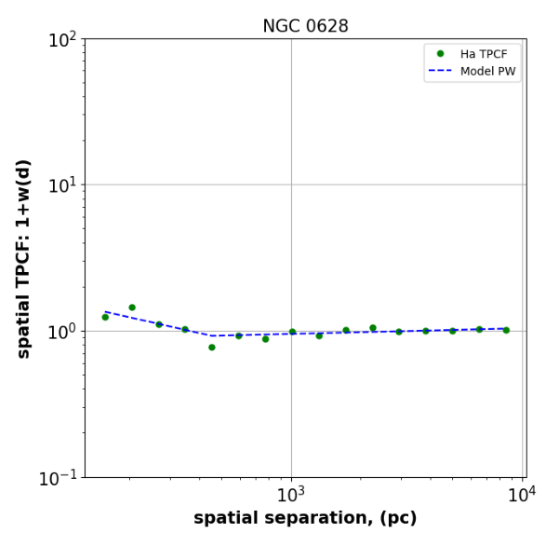
\includegraphics[scale = 0.5]{image1.png}
        \caption{Without the cut}
        \label{fig:tpcf_without_cut}
    \end{subfigure}
    ~
    \begin{subfigure}{0.45\textwidth}
        \centering
        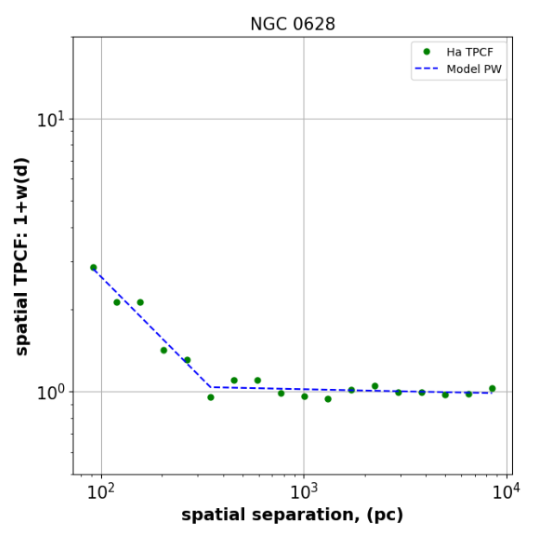
\includegraphics[scale = 0.5]{image2.png}
        \caption{With the cut}
        \label{fig:tpcf_with_cut}
    \end{subfigure}
    \caption{TPCF plots of NGC 628}
\end{figure}

There are two plots in the figure above. The plot on the left is the TPCF plot of NGC 628 as obtained without the cut. The plot on the right is the TPCF plot of NGC 628 as obtained with the cut. The cut is a threshold value that was set on the luminosity and ionization parameter of the stars. \\

\textit{\textbf{Luminosity (L)} is the total amount of energy emitted by a star per unit time. It has units of watts and is calculated from the flux through the formula: $L = 4\pi d^2 F$, where $d$ is the distance of the star from the observer and $F$ is the flux.}

\textit{The \textbf{Ionization Parameter (U)} is a measure of the ionizing radiation field of a star. It is defined as the ratio of the number density of ionizing photons to the number density of hydrogen atoms} \\

For the right plot, the cut was set at $L \ge 10^{37}$ erg/s and $\log U \ge 6.5$. This effectively helps us isolate the younger HII regions in NGC 628. We observe that the TPCF plot with the cut shows a higher correlation at smaller scales, indicating that younger regions are more likely to show hierarchical structures than older regions. 

My work takes direct inspiration from Nimya's work, and aims to develop a better way to characterize these different HII regions based on their age, which in turn will help us gain a better understanding of these cuts and the factors that affect their hierarchical distribution. 

\section{Age Estimation of HII Regions}

The age of a star forming region is an important parameter that can provide insights into the physical processes involved in star formation. There are different ways to estimate the age of a star forming region, the most common one being the \textbf{SED fitting} method. \\

\textit{The \textbf{Spectral Energy Distribution (SED)} of a star is the distribution of energy emitted by the star at different wavelengths. It is a plot of the energy emitted by the star as a function of wavelength. }\\

The SED fitting method involves fitting the observed SED of a star forming region with theoretical models of star formation to estimate the age of the region. However, one of the major flaws in this method is that it might incorrectly estimate the age of an older regions with less \textbf{extinction} as younger regions with more extinction and vice versa.\\

\textit{\textbf{Extinction} is the process by which the light from a star is scattered by dust grains in the interstellar medium, leading to a decrease in the observed flux of the star. This is more prominent in lower wavelengths as they are more energetic and so are scattered more easily by the dust grains.}\\

If we can model the variation of other parameters of these HII regions along with the age, we can overcome this limitation and obtain more accurate age estimates. A list of such possible parameters is given below:

\begin{itemize}
    \item Luminosity
    \item Ionization Parameter
    \item Equivalent Width of H$\alpha$ line \\
\end{itemize}

\textit{The \textbf{Equivalent Width (EW)} of a spectral line is a measure of the strength of the line. It is defined as the width of a rectangle with the same area as the line profile, as shown in the figure below:}

\begin{figure}[H]
    \centering
    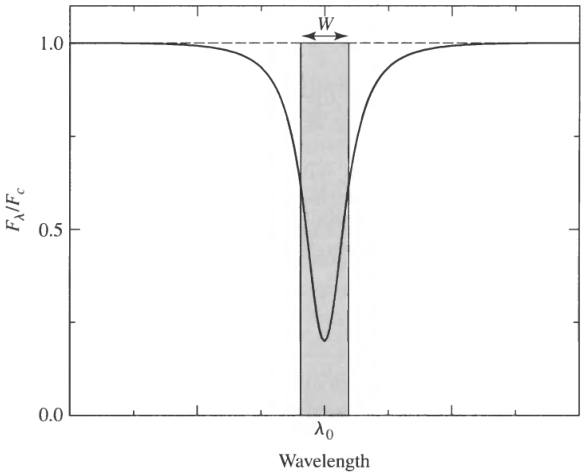
\includegraphics[scale = 0.5]{image3.png}
    \caption{Equivalent Width (W) of a spectral line (\textit{Carroll and Ostlie, 2007})}
    \label{fig:image3}
\end{figure}

\textit{ It is given by the formula $EW = \int (1 - \frac{F(\lambda)}{F_{\text{cont}}}) d\lambda$, where $F(\lambda)$ is the flux of the line at wavelength $\lambda$ and $F_{\text{cont}}$ is the continuum flux.}\\

The main objective of this project is to experiment and compare the different possible age estimators for young star forming regions, and study their variation with other parameters as well as their effectiveness in characterizing the age distribution of young stars. We aim to understand how these age estimators can be used to study the properties of young star forming regions and consequently, the hierarchical structure of star formation.

\chapter{Analysis}

\section{Correlation Analysis of Age Estimators in PHANGS Galaxies}

My first task was to analyze the relationship between the different age estimators amongst themselves. For this, I used the data from the PHANGS-MUSE HII Regions Catalogue \cite{santoro2022phangs} and the PHANGS Nebular Catalogue \cite{groves2023phangs} which contained the required data for 19 Galaxies in the PHANGS survey. The data included the different age estimators, the luminosity, the ionization parameter, and the equivalent width of the H$\alpha$ line for each HII region which we were interested in.

Upon plotting the different age estimators against each other, I found that the age estimators were not consistent with each other across multiple galaxies. This was evident from the scatter plots of the different age estimators against each other that can be seen in Figure \ref{fig:grid_of_images}. For galaxies like NGC0628, the age estimators showed good correlation with each other, while for galaxies like NGC1566 and NGC1433, the correlations between the age estimators were not as strong. 

It is however important to note that a strong correlation between equivalent width and luminosity was observed in all the galaxies. This is consistent with the fact that the equivalent width of the H$\alpha$ line is a measure of the strength of the line, and is directly related to the luminosity, as higher the luminosity, greater the line peak and hence the equivalent width.

Now, upon further applying the luminosity and ionization parameter that was used by Nimya, I found that the age estimators showed a better correlation with each other. This is evident from the scatter plots shown in Figure \ref{fig:grid_of_images_with_cuts}. This further strengthens the hypothesis that the luminosity and ionization parameter can be used to isolate the younger HII regions in a galaxy, and that the age estimators show a better correlation with each other in these regions.


\begin{figure}[htbp]
    \centering
    
    \caption*{NGC0628}
    \begin{subfigure}{0.3\textwidth}
        \centering
        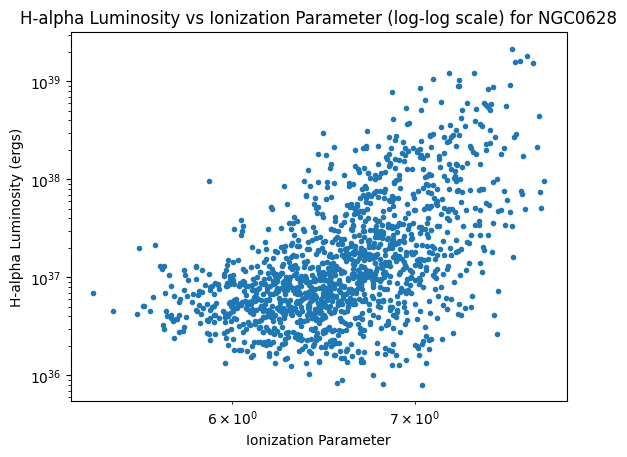
\includegraphics[width=\linewidth]{image4.png}
        % \caption{Image 4}
        \label{fig:image4}
    \end{subfigure}
    \hfill
    \begin{subfigure}{0.3\textwidth}
        \centering
        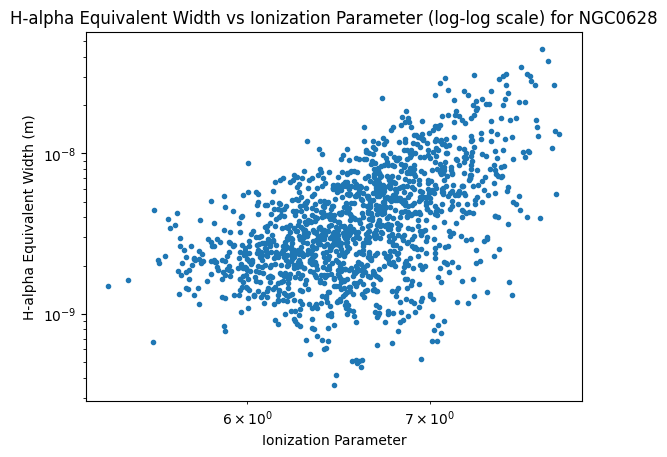
\includegraphics[width=\linewidth]{image5.png}
        % \caption{Image 5}
        \label{fig:image5}
    \end{subfigure}
    \hfill
    \begin{subfigure}{0.3\textwidth}
        \centering
        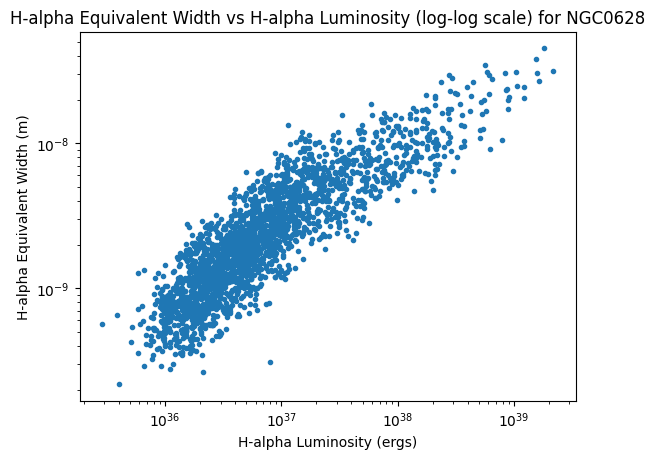
\includegraphics[width=\linewidth]{image6.png}
        % \caption{Image 6}
        \label{fig:image6}
    \end{subfigure}

    
    \vspace{0.5cm}
    \caption*{NGC1566}
    
    \begin{subfigure}{0.3\textwidth}
        \centering
        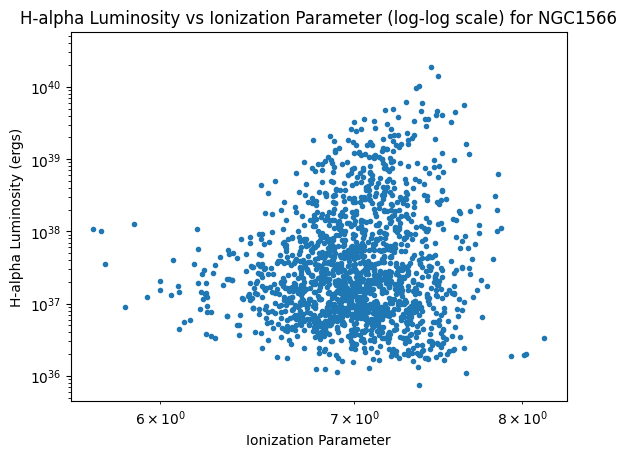
\includegraphics[width=\linewidth]{image7.png}
        % \caption{Image 7}
        \label{fig:image7}
    \end{subfigure}
    \hfill
    \begin{subfigure}{0.3\textwidth}
        \centering
        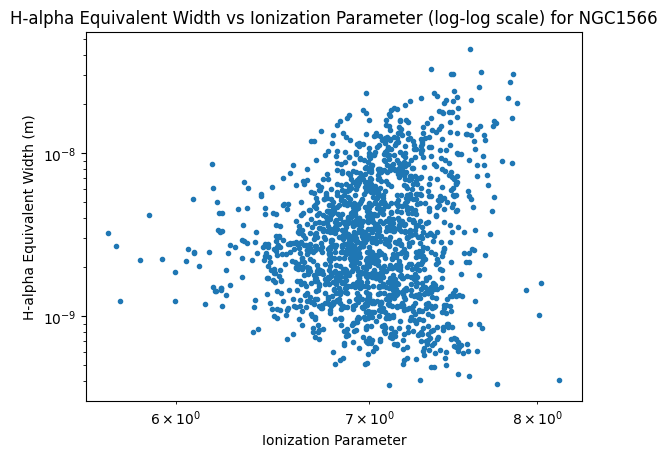
\includegraphics[width=\linewidth]{image8.png}
        % \caption{Image 8}
        \label{fig:image8}
    \end{subfigure}
    \hfill
    \begin{subfigure}{0.3\textwidth}
        \centering
        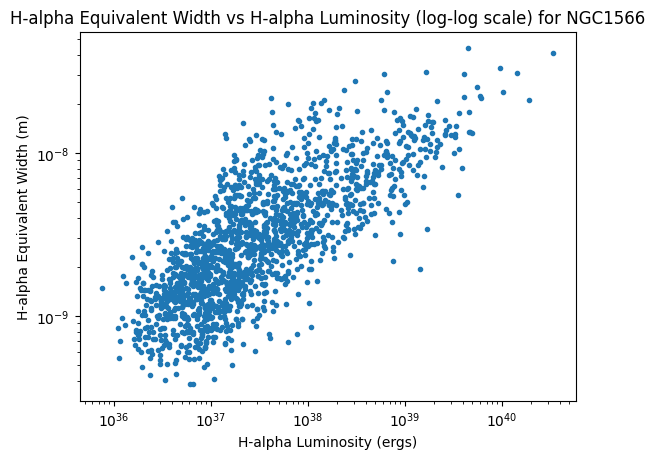
\includegraphics[width=\linewidth]{image9.png}
        % \caption{Image 9}
        \label{fig:image9}
    \end{subfigure}
    
    \vspace{0.5cm}
    \caption*{NGC1433}
    
    \begin{subfigure}{0.3\textwidth}
        \centering
        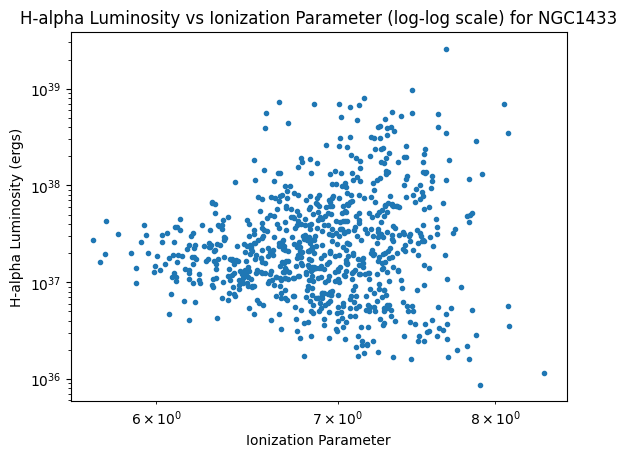
\includegraphics[width=\linewidth]{image10.png}
        % \caption{Image 10}
        \label{fig:image10}
    \end{subfigure}
    \hfill
    \begin{subfigure}{0.3\textwidth}
        \centering
        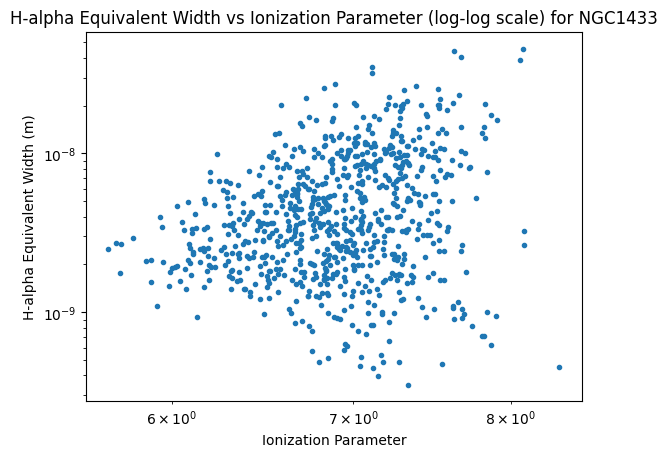
\includegraphics[width=\linewidth]{image11.png}
        % \caption{Image 11}
        \label{fig:image11}
    \end{subfigure}
    \hfill
    \begin{subfigure}{0.3\textwidth}
        \centering
        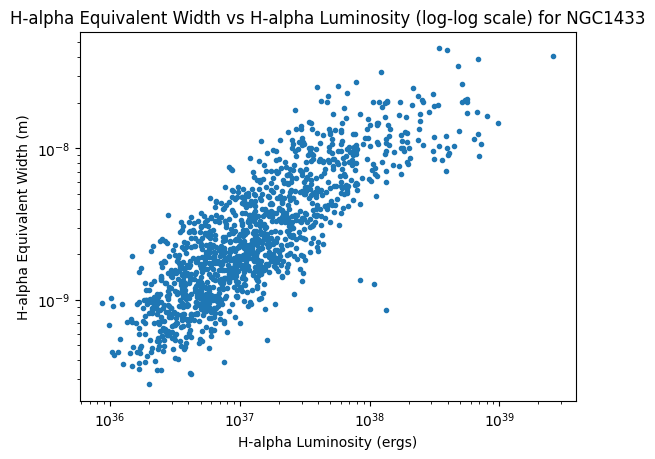
\includegraphics[width=\linewidth]{image12.png}
        % \caption{Image 12}
        \label{fig:image12}
    \end{subfigure}
    
    \small
    \caption{Scatter plots of H$\alpha$ Equivalent Width, Luminosity, and Ionization Parameter against each other for the galaxies NGC0628, NGC1566, and NGC1433}
    \label{fig:grid_of_images}
\end{figure}


\begin{figure}[htbp]
    \centering

    \begin{subfigure}{0.3\textwidth}
        \centering
        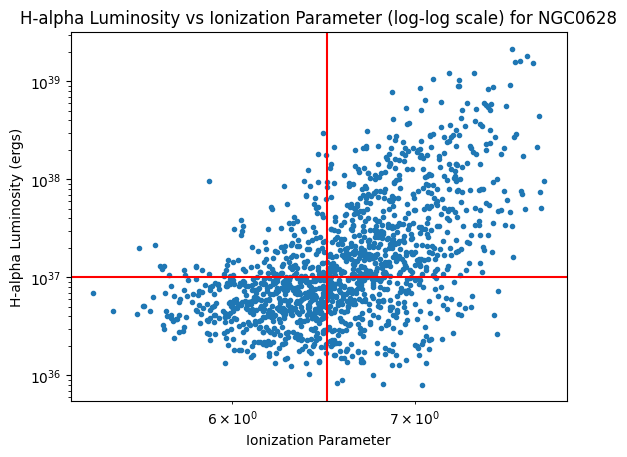
\includegraphics[width=\linewidth]{image13.png}
        \caption{NGC0628}
        \label{fig:image13}
    \end{subfigure}
    \hfill
    \begin{subfigure}{0.3\textwidth}
        \centering
        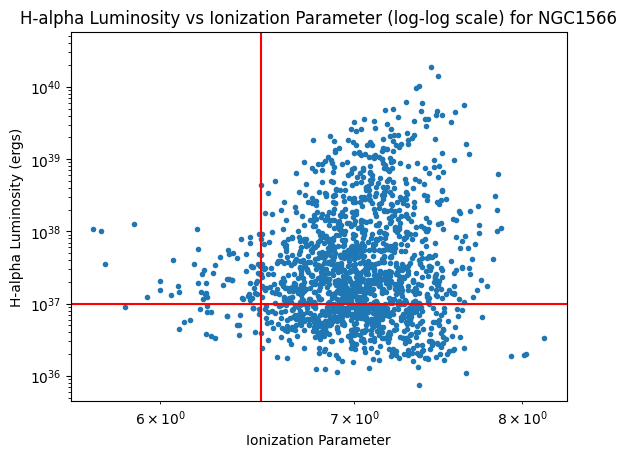
\includegraphics[width=\linewidth]{image14.png}
        \caption{NGC1566}
        \label{fig:image14}
    \end{subfigure}
    \hfill
    \begin{subfigure}{0.3\textwidth}
        \centering
        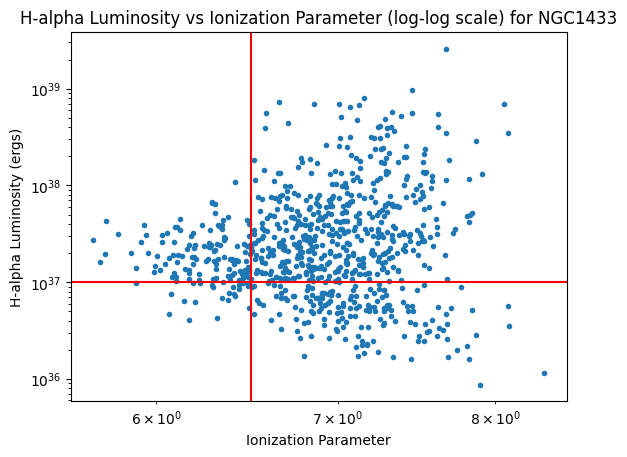
\includegraphics[width=\linewidth]{image15.png}
        \caption{NGC1433}
        \label{fig:image15}
    \end{subfigure}

    \small
    \caption{Scatter plots of H$\alpha$ luminosity and ionization parameter against each other for the galaxies NGC0628, NGC1566, and NGC1433 with the cuts applied}
    \label{fig:grid_of_images_with_cuts}

\end{figure}

\section{Correlation Analysis and Age Estimation with Insights from Scheuermann et al. (2023)}

Next, I wanted to take a closer look into a similar analysis that was done by Scheuermann et al. \cite{scheuermann2023stellar}. They used the data from the PHANGS-MUSE survey to identify HII regions and the PHANGS-HST survey to identify the stellar associations observed in these regions. Upon identifying the HII regions and the stellar associations, they filtered out the regions that were not associated with any stellar association, and used only the HII regions which had a single completely contained stellar association for their analysis. 

The correlation analysis of the age estimators in these regions showed a much more consistent correlation between the age estimators across the different galaxies, which was expected but not observed in the previous analysis. 

\begin{figure}[htbp]
    \centering
    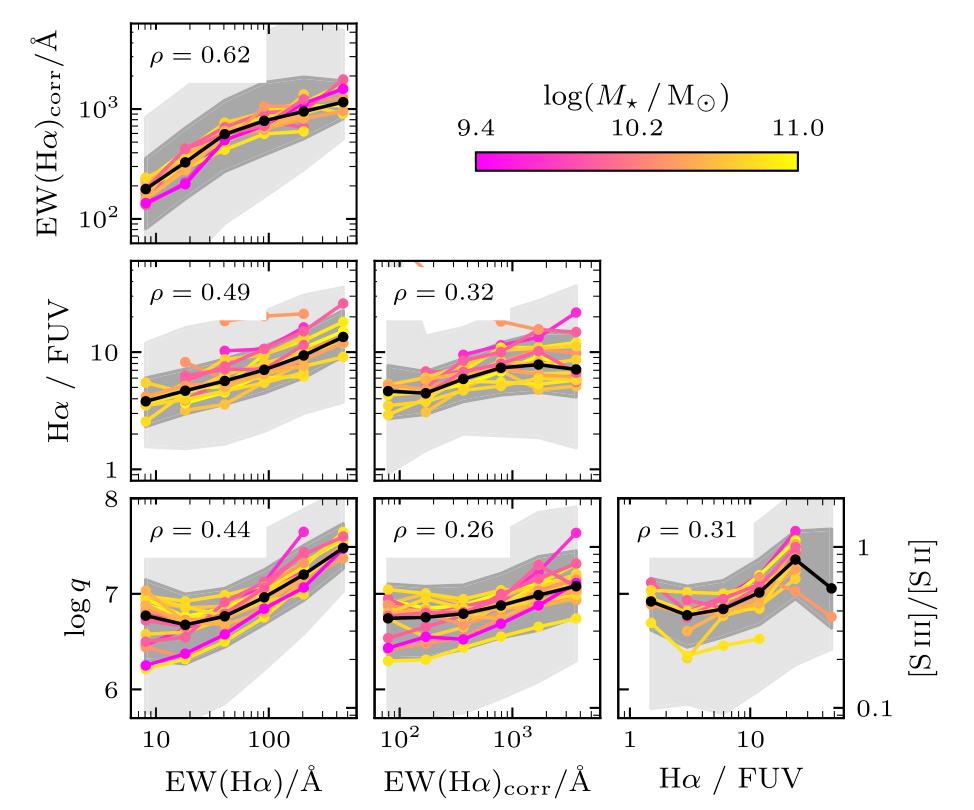
\includegraphics[scale = 0.45]{image16.png}
    \caption{Plots of the different age estimators against each other for the associated HII regions (\textit{Scheuermann et al., 2023})}
    \label{fig:image16}
\end{figure}

Further, they also calculated the ages of these stellar associations using the SED fitting method, and compared the ages of the HII regions and the stellar associations. Upon plotting the potential age estimators against the SED ages (Figure \ref{fig:image17}), they found that initially there is a good drop in the age estimators as the SED age increases (which is expected, as a region ages the ionization parameter, luminosity, and equivalent width of the H$\alpha$ line decrease), but after a certain point, the age estimators start to increase again. This is contrary to what is expected, and indicates possible errors in the age estimation of these regions. 

\begin{figure}[H]
    \centering
    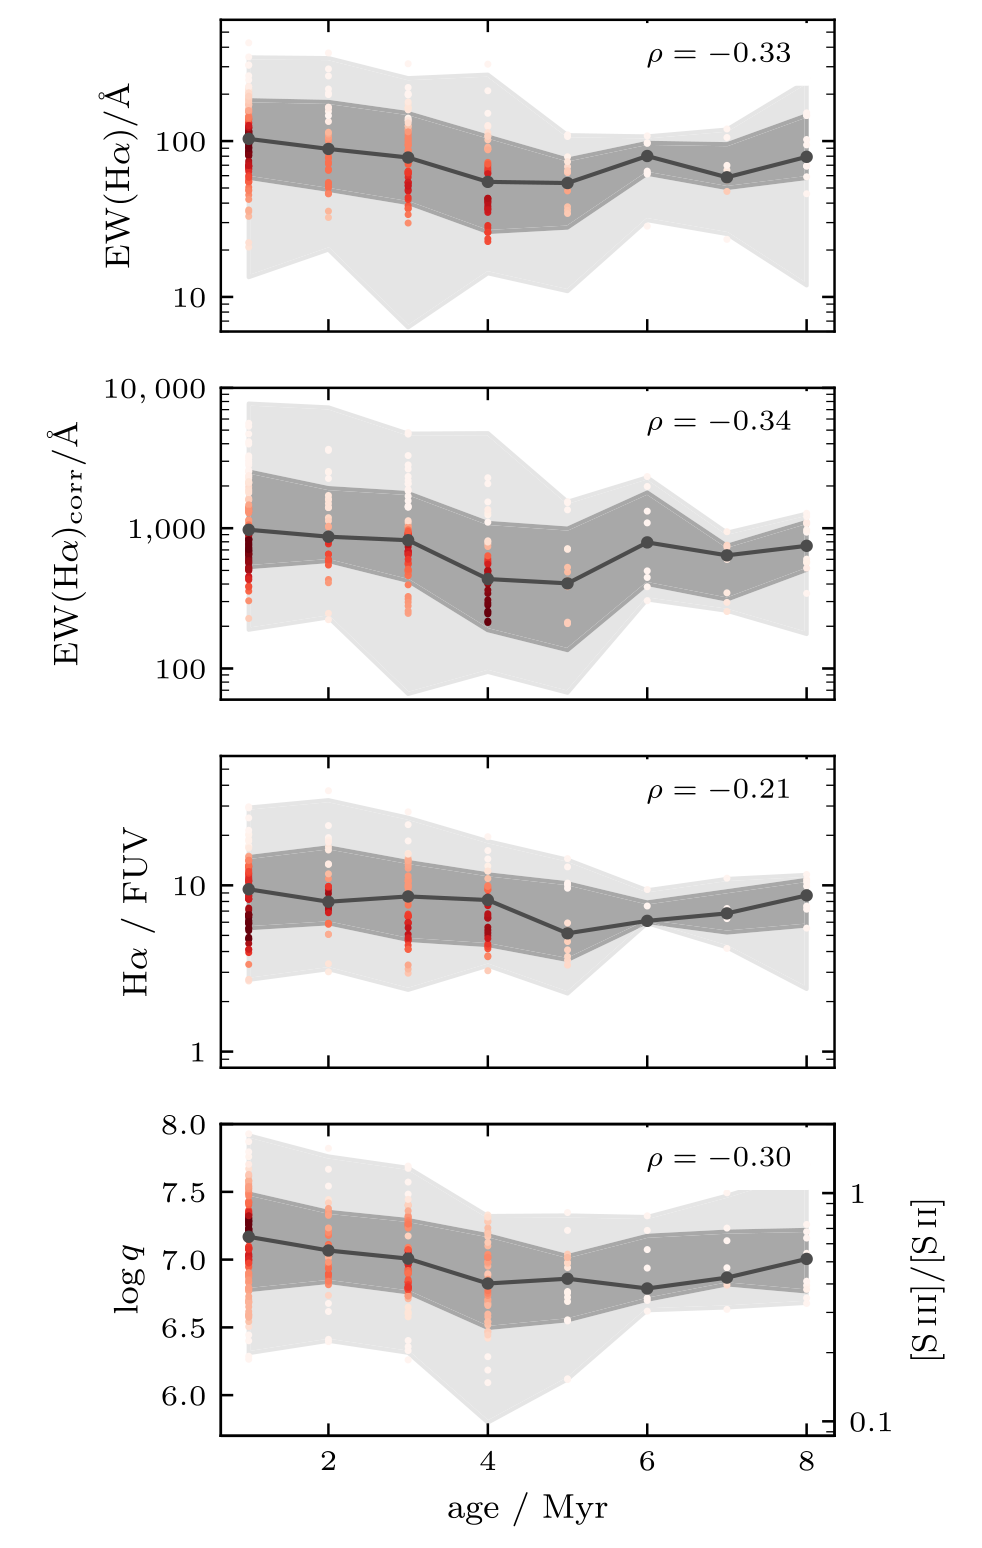
\includegraphics[scale = 0.3]{image17.png}
    \caption{Plots of the age estimators against the SED ages for the associated HII regions (\textit{Scheuermann et al., 2023})}
    \label{fig:image17}
\end{figure}


However, analysis done by Scheuermann et al. was limited to within 6 Myr of the SED age, and so to check if this trend continues beyond this range, I plotted the age estimators against the SED ages for an extended range of 40 Myr using their compiled data. The results dont show a clear trend, but an overall dip in the age estimators as the SED age increases is observed. This indicates that the age estimators are consistent with the SED ages for the most part, but there are some discrepancies that need to be addressed.


\begin{figure}[htbp]
    \centering

    \begin{subfigure}{0.4\textwidth}
        \centering
        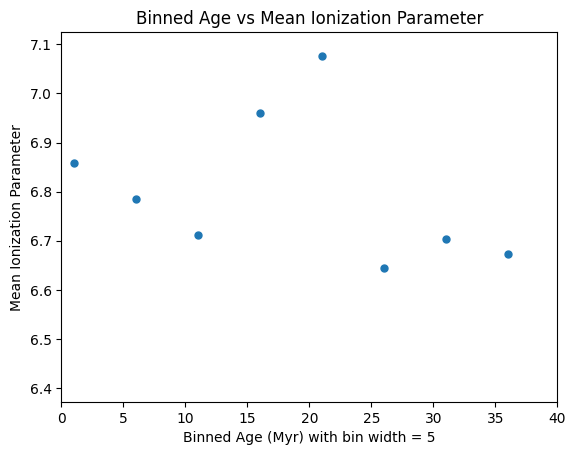
\includegraphics[width=\linewidth]{image18.png}
        % \caption{}
        \label{fig:image18}
    \end{subfigure}
    \hfill
    \begin{subfigure}{0.4\textwidth}
        \centering
        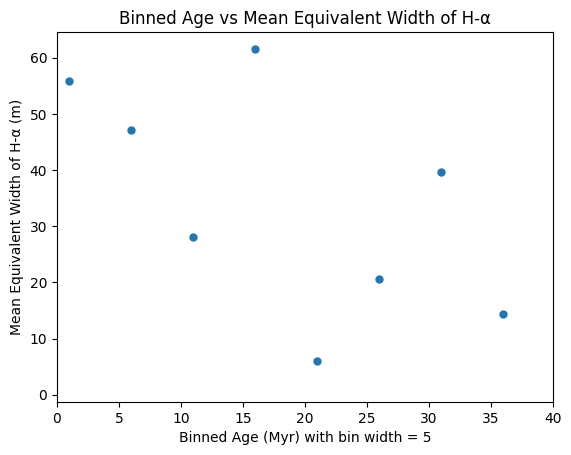
\includegraphics[width=\linewidth]{image19.png}
        % \caption{}
        \label{fig:image19}
    \end{subfigure}

    \small
    \caption{Plots of the age estimators against the SED ages for the associated HII regions for an extended range of 40 Myr}
    \label{fig: image18_19}
\end{figure}


One such discrepancy comes from the possibility that the SED ages are not accurate due to the incorrect estimation of the extinction. The extinction is a crucial parameter in the SED fitting method, and an incorrect estimation of the extinction can lead to an incorrect estimation of the age. This is evident in a plot of the extinction calculated through the SED fitting method against the extinction calculated through the Balmer decrement method (Figure \ref{fig:image21}). 

\vspace*{0.6cm}
\textit{The \textbf{Balmer Decrement} is the ratio of the flux of the H$\alpha$ line to the H$\beta$ line. It is used to estimate the extinction in a star forming region, as the ratio of the flux of these two lines is expected to be constant.}\\

\begin{figure}[htbp]
    \centering
    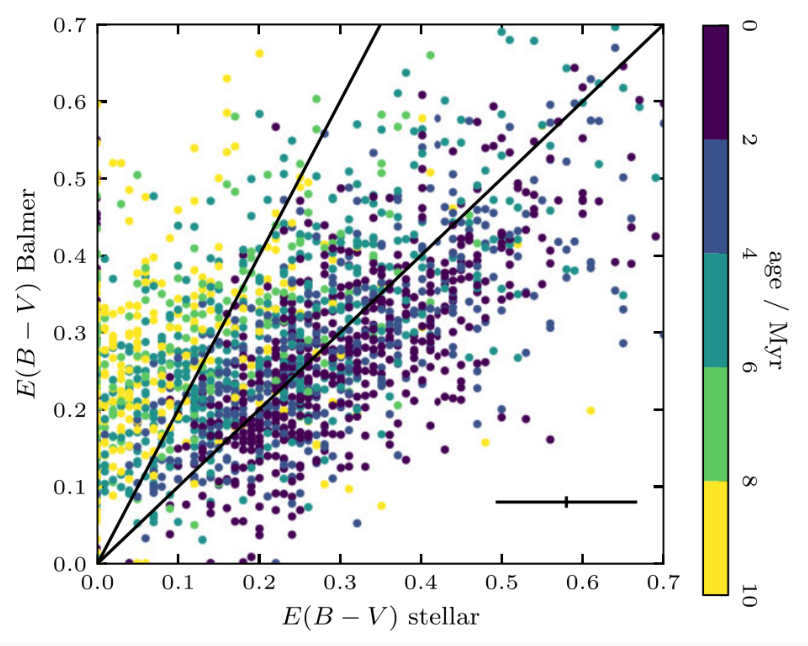
\includegraphics[scale = 0.4]{image21.png}
    \caption{Plot of the extinction calculated through the SED fitting method against the extinction calculated through the Balmer decrement method (\textit{Scheuermann et al., 2023})}
    \label{fig:image21}
\end{figure}

The plot shows that for lower ages, the extinction calculated through both methods are in good correlation with each other, but as the age increases, the extinction calculated through the SED fitting method starts to deviate from the extinction calculated through the Balmer decrement method. This indicates that the SED ages might not be accurate and that the extinction might be incorrectly estimated in these regions.

The paper concludes that the age estimators are consistent with the SED ages for the most part, but there are some discrepancies that need to be addressed. Out of all the age estimators, the equivalent width of the H$\alpha$ line showed the best correlation with the SED ages, and so it can be a potential age tracer for young star forming regions. 

\section{Evolution of Age Estimators in NGC1566 Using UVIT Data}

The analysis done by Scheuermann et al. \cite{scheuermann2023stellar} provided valuable insights, but the discrepancy in the SED ages was a major limitation. To address this, I decided to use the UVIT data from AstroSat to estimate the ages of the stellar associations in the galaxy NGC1566. 

The UVIT data from AstroSat was downloaded from the AstroSat Archive and the data analysis was done using the \href{https://youtu.be/QyIfjwN4DK4?si=G0OCJarjRbgJhqsX}{UVIT pipeline}  in CCDLAB \cite{postma2017ccdlab} which is a software package for the analysis of FITS files and the extraction of photometric data. The UVIT data contained the flux of the stars in the FUV, NUV and VIS bands, which was used in the analysis. The data reduction pipeline included the following steps (Figure \ref{fig:UVIT_pipeline}):

\begin{itemize}
    \item Drift correction was performed using the VIS band data to correct for the drift in the telescope.
    \item Registration of the FUV and NUV data with the VIS data was done to align the images.
    \item WCS coordinates were extracted to obtain the RA and DEC of the stars.
    \item Final photometry was done to obtain the flux of the stars in the FUV, NUV and VIS bands.
\end{itemize}

\begin{figure}[htbp]
    \centering

    \begin{subfigure}{0.45\textwidth}
        \centering
        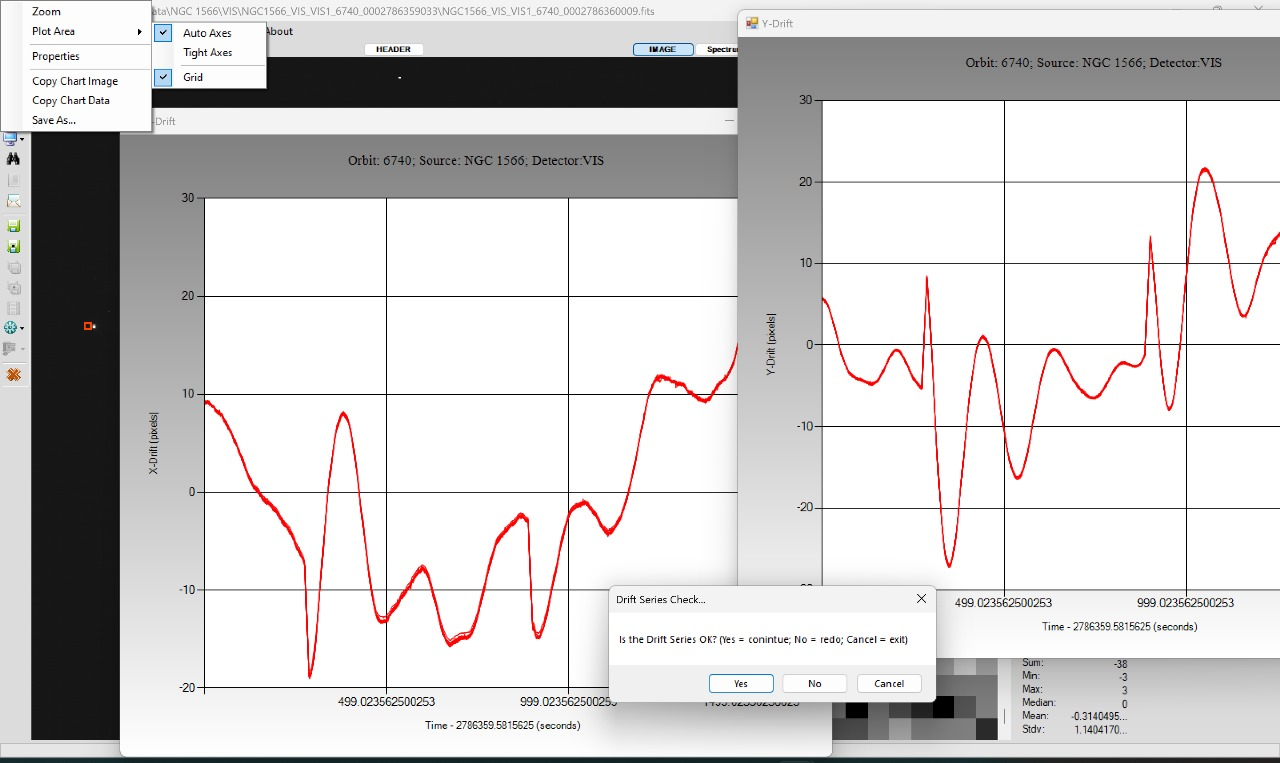
\includegraphics[width=\linewidth]{image28.png}
        % \caption{}
        \label{fig:image28}
    \end{subfigure}
    \hfill
    \begin{subfigure}{0.45\textwidth}
        \centering
        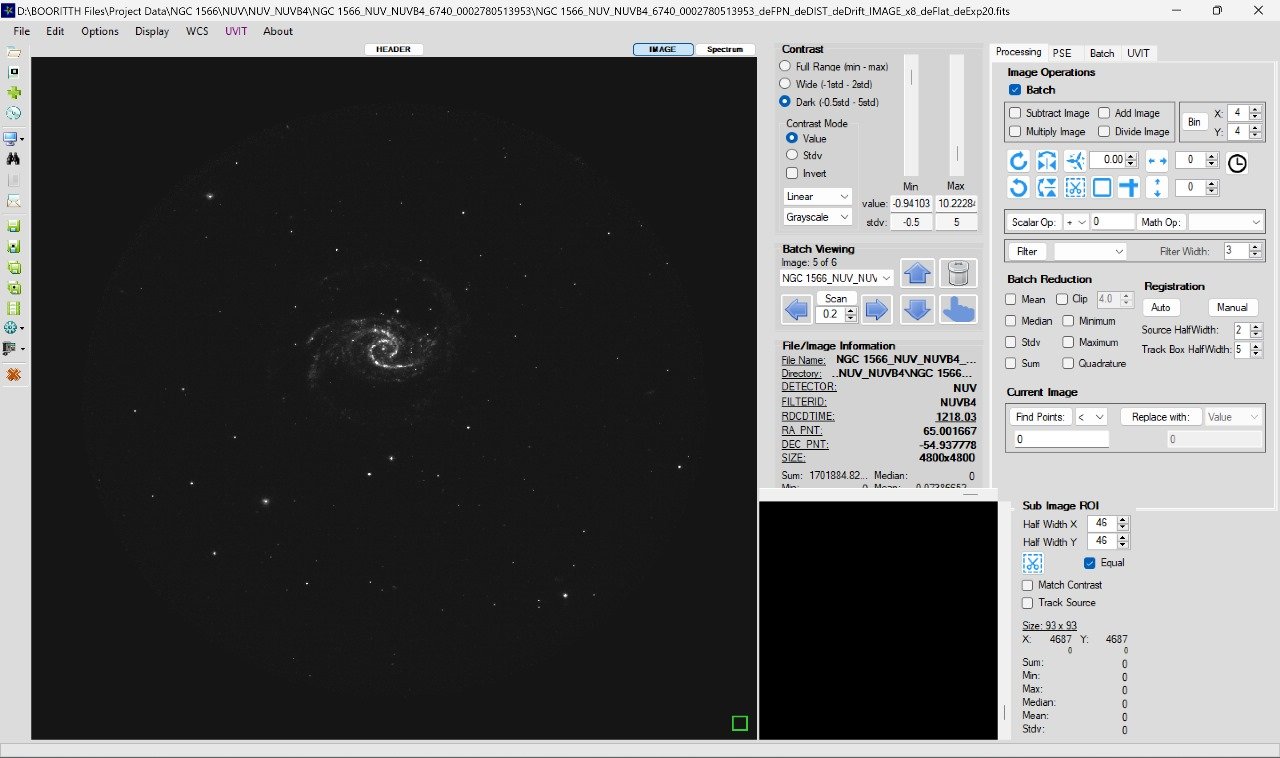
\includegraphics[width=\linewidth]{image29.png}
        % \caption{}
        \label{fig:image29}
    \end{subfigure}
    \label{fig: image2829}
    \caption*{Drift Correction}


    \begin{subfigure}{0.45\textwidth}
        \centering
        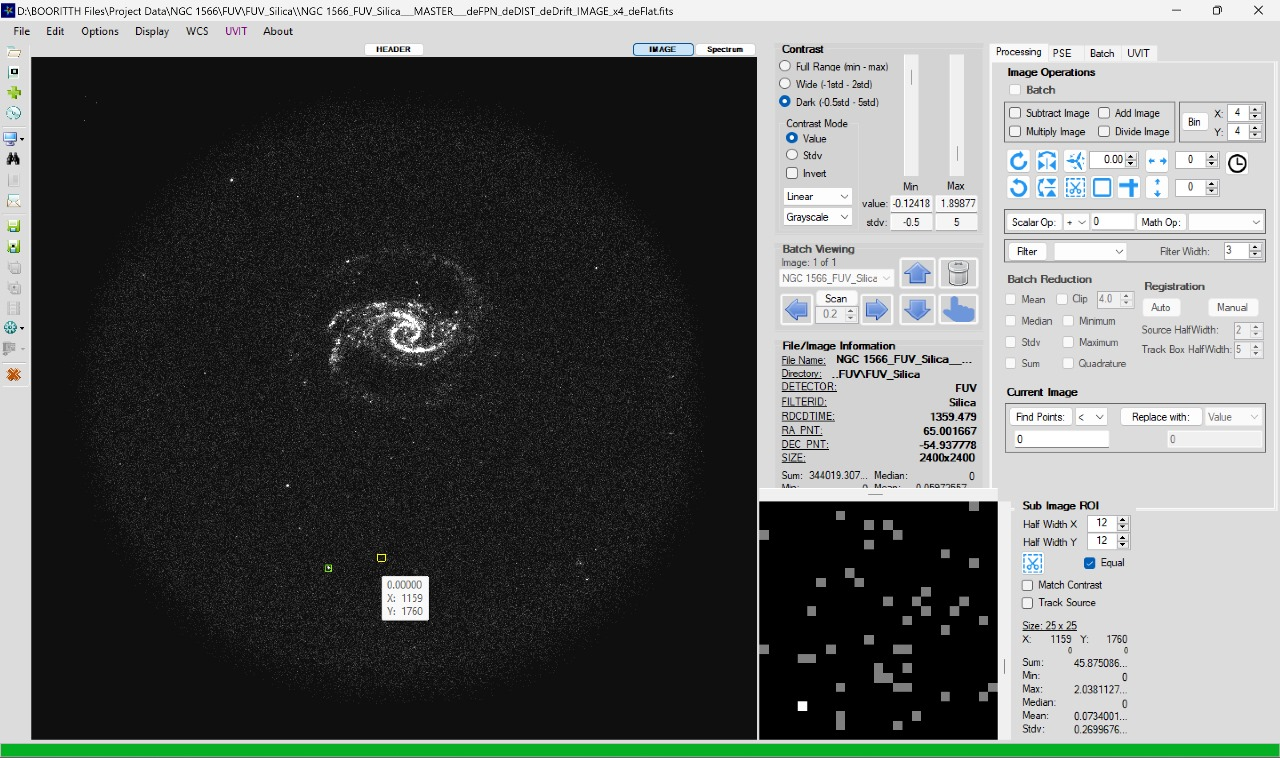
\includegraphics[width=\linewidth]{image30.png}
        % \caption{}
        \label{fig:image30}
    \end{subfigure}
    \hfill
    \begin{subfigure}{0.45\textwidth}
        \centering
        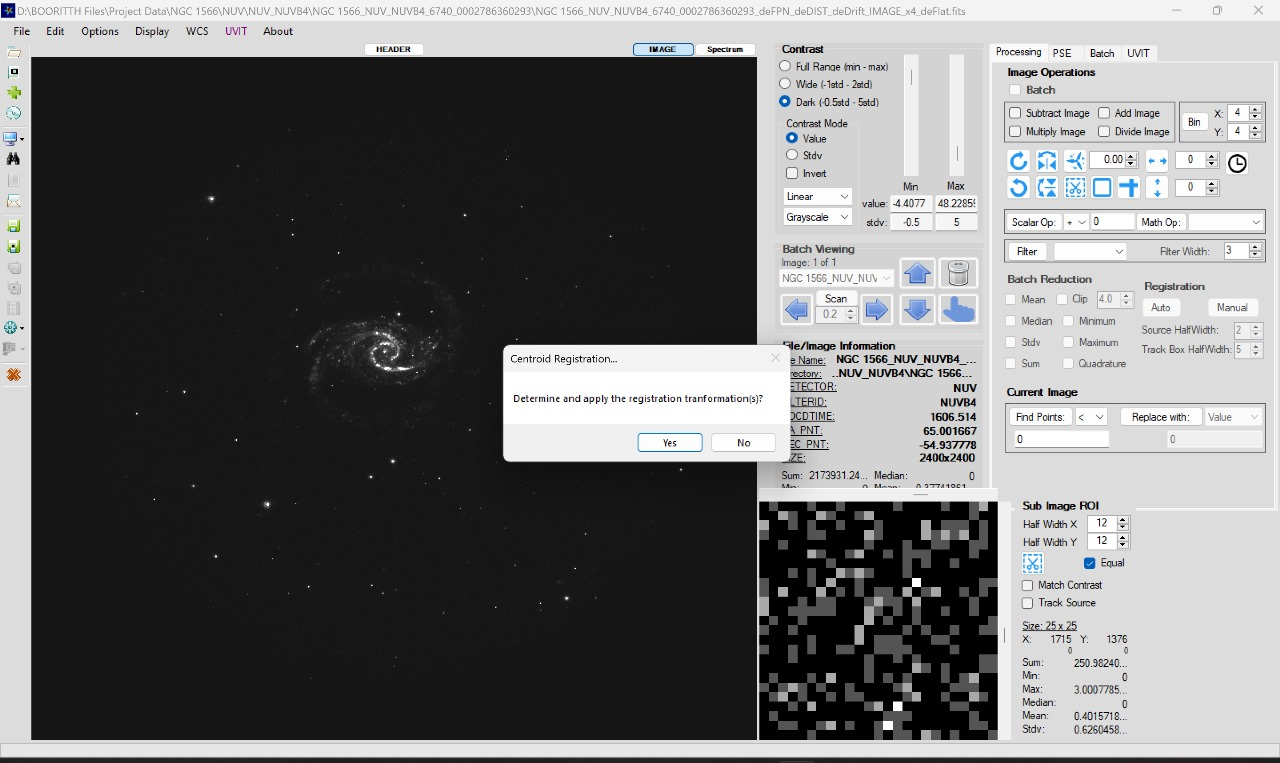
\includegraphics[width=\linewidth]{image31.png}
        % \caption{}
        \label{fig:image31}
    \end{subfigure}
    \caption*{Registration of UV with VIS and image alignment}

    \begin{subfigure}{0.45\textwidth}
        \centering
        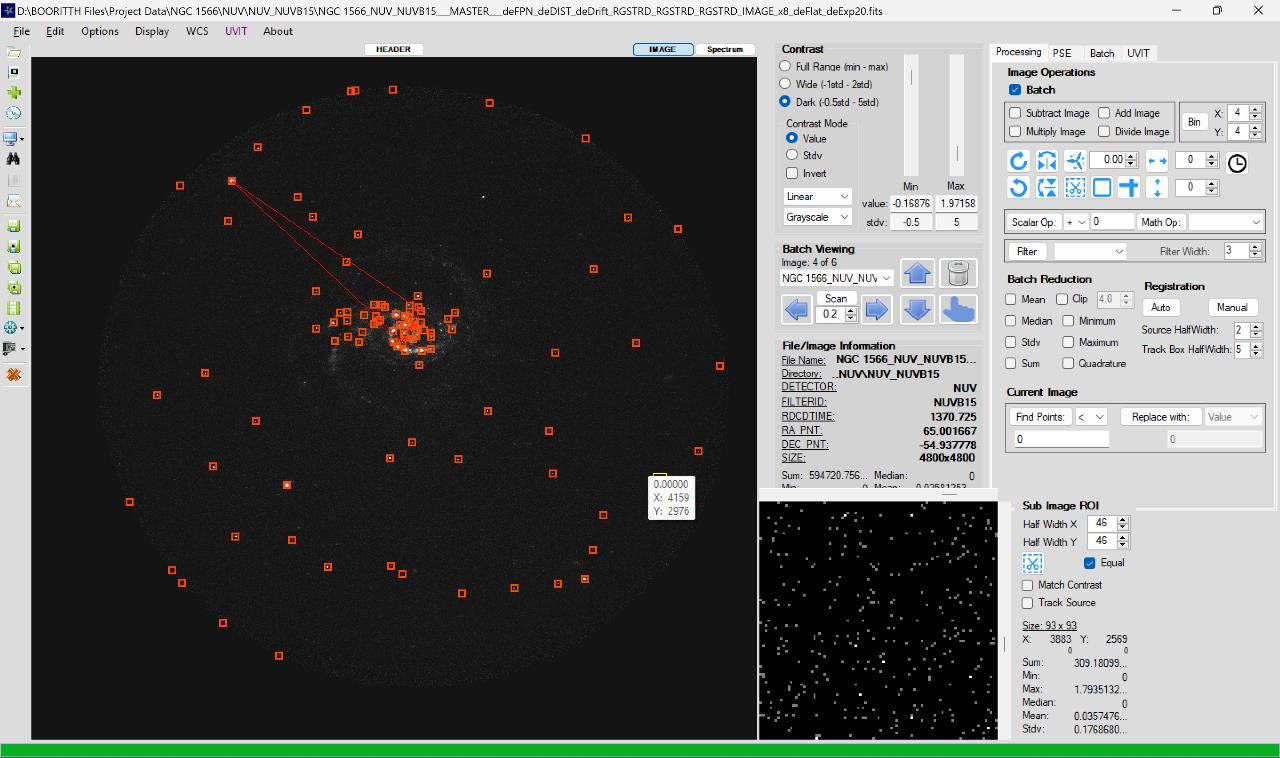
\includegraphics[width=\linewidth]{image32.png}
        % \caption{}
        \label{fig:image32}
    \end{subfigure}
    \hfill
    \begin{subfigure}{0.45\textwidth}
        \centering
        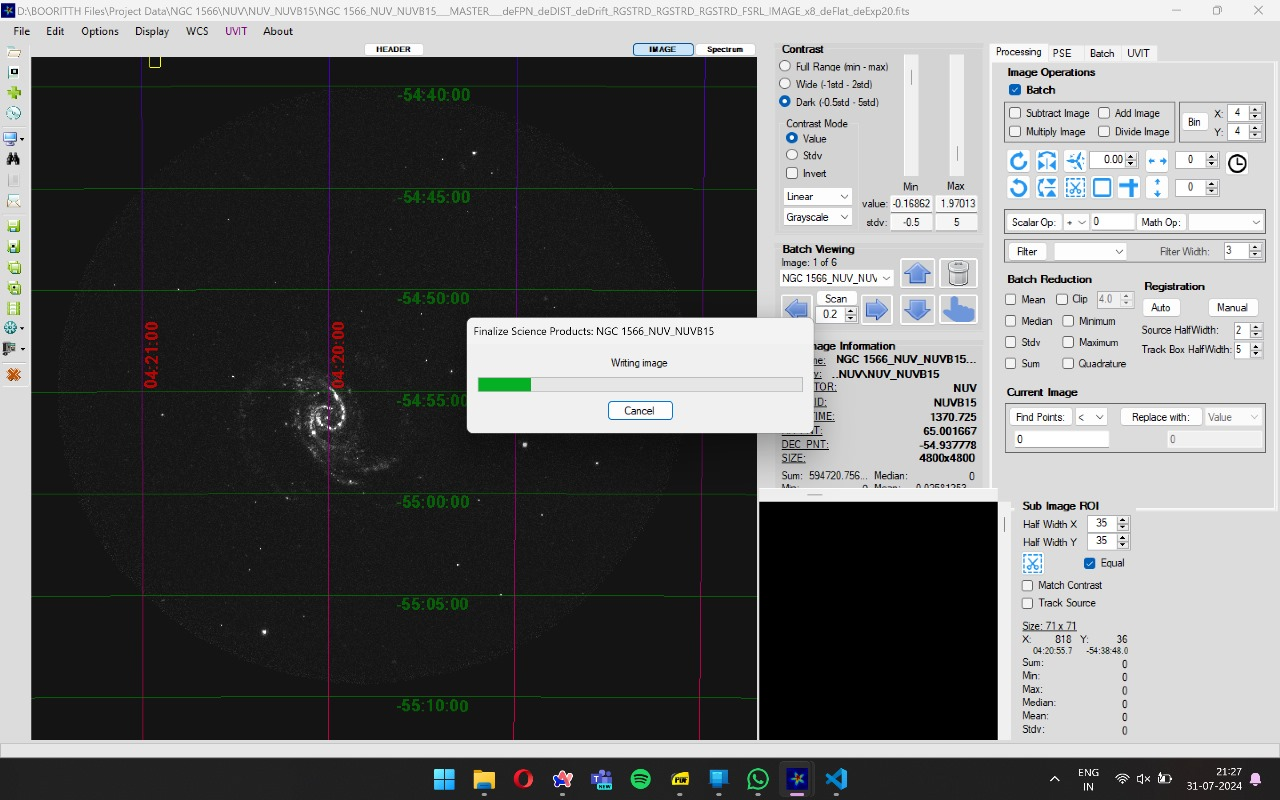
\includegraphics[width=\linewidth]{image34.png}
        % \caption{}
        \label{fig:image34}
    \end{subfigure}
    \caption*{WCS Coordinates Extraction and Finalizing Science Products}

    \small
    \caption{Snapshots of the UVIT data reduction pipeline for NGC1566 in CCDLAB}
    \label{fig:UVIT_pipeline}

\end{figure}




The UVIT data was then processed further by Shashank Gairola and compared to the models generated through StarBurst99 to estimate the ages of the stellar associations in NGC1566. This data was then cross matched with the HII regions in NGC1566 from my previous analysis using TOPCAT with an error radius of 1.5 arcseconds and the evolution of the age estimators with the calculated ages was studied.

The results shown in Figure \ref{fig:UVIT_ages} show an overall decrease in the ionization parameter as the age increases, but the equivalent width of the H$\alpha$ line shows a more scattered trend. This indicates that the equivalent width of the H$\alpha$ line might not be a reliable age estimator for young star forming regions. 

\begin{figure}[htbp]
    \centering

    \begin{subfigure}{0.45\textwidth}
        \centering
        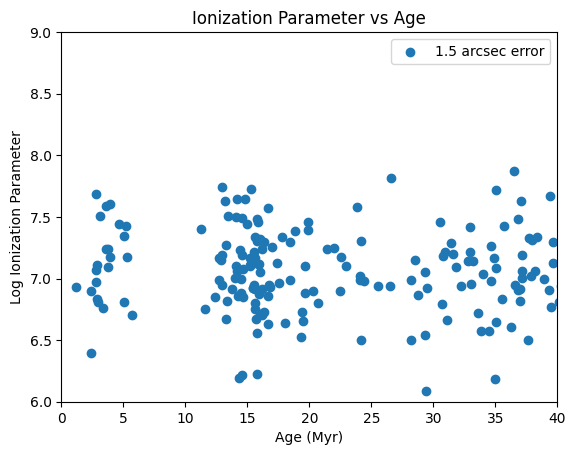
\includegraphics[width=\linewidth]{image22.png}
        % \caption{}
        \label{fig:image22}
    \end{subfigure}
    \hfill
    \begin{subfigure}{0.45\textwidth}
        \centering
        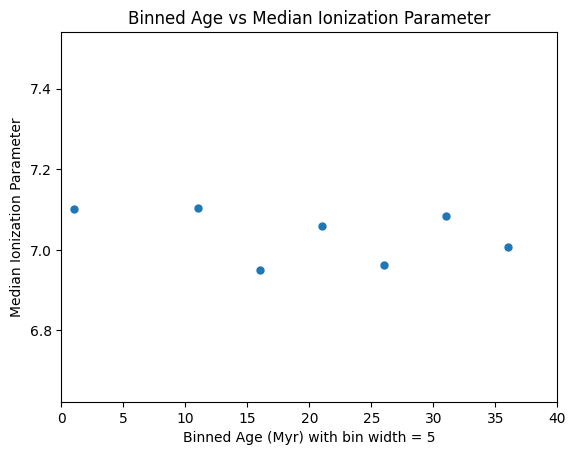
\includegraphics[width=\linewidth]{image24.png}
        % \caption{}
        \label{fig:image24}
    \end{subfigure}
    \label{fig: image2224}


    \begin{subfigure}{0.45\textwidth}
        \centering
        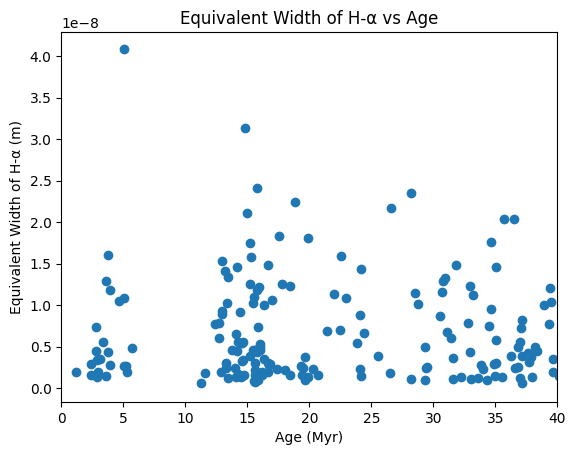
\includegraphics[width=\linewidth]{image23.png}
        % \caption{}
        \label{fig:image23}
    \end{subfigure}
    \hfill
    \begin{subfigure}{0.45\textwidth}
        \centering
        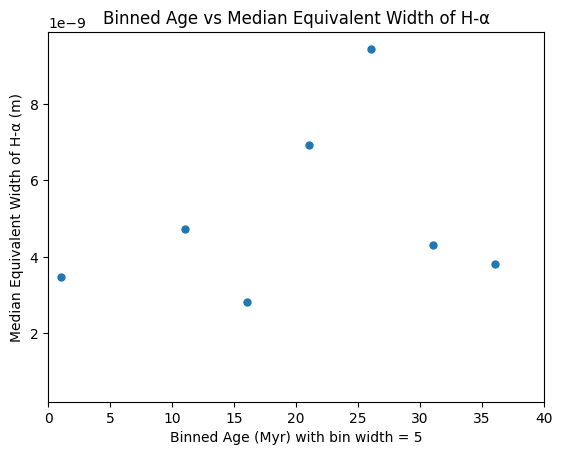
\includegraphics[width=\linewidth]{image25.png}
        % \caption{}
        \label{fig:image25}
    \end{subfigure}

    \begin{subfigure}{0.45\textwidth}
        \centering
        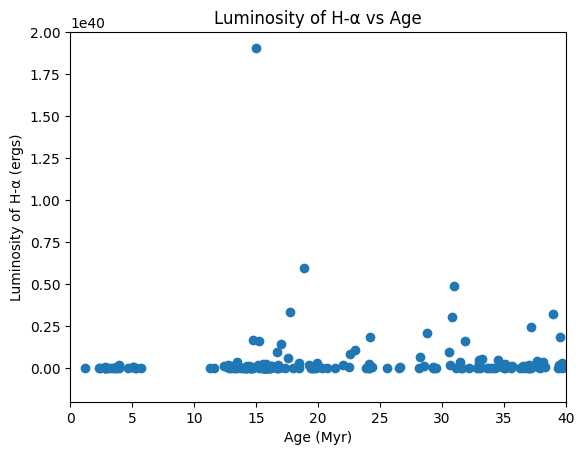
\includegraphics[width=\linewidth]{image26.png}
        % \caption{}
        \label{fig:image26}
    \end{subfigure}
    \hfill
    \begin{subfigure}{0.45\textwidth}
        \centering
        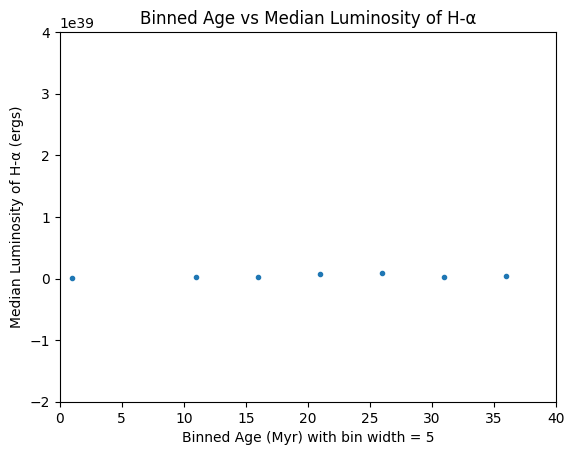
\includegraphics[width=\linewidth]{image27.png}
        % \caption{}
        \label{fig:image27}
    \end{subfigure}

    \small
    \caption{Plots of the age estimators against binned UVIT/StarBurst99 ages for NGC1566 with and without binning}
    \label{fig:UVIT_ages}

\end{figure}



\chapter{Results and Conclusions}

The analysis of the age estimators in the PHANGS galaxies showed that the age estimators were not consistent with each other across multiple galaxies, but showed a better correlation with each other when the luminosity and ionization parameter were applied. This indicates that the luminosity and ionization parameter can be used to isolate the younger HII regions in a galaxy, and that the age estimators show a better correlation with each other in these regions.\\

The analysis done by Scheuermann et al. \cite{scheuermann2023stellar} provided valuable insights into the correlation between the age estimators and the SED ages, but the discrepancy in the SED ages was a major limitation. The analysis showed that the age estimators are consistent with the SED ages for the most part, but there are some discrepancies that need to be addressed mainly the incorrect estimation of the extinction, which can lead to a false estimation of age and consequently the trends observed in the age estimators. Out of all the age estimators, the equivalent width of the H$\alpha$ line showed the best correlation with the SED ages, and so it can be a potential age tracer for young star forming regions.\\

The analysis of the UVIT data from AstroSat showed an overall decrease in the ionization parameter as the age increases, but the equivalent width of the H$\alpha$ line showed a more scattered trend. \\

The results of this project indicate that the age estimators are consistent for the most part, however further analysis must be done before they can be used as reliable age tracers for young star forming regions. The most reliable age estimator was found to be the equivalent width of the H$\alpha$ line followed by the ionization parameter, while the H$\alpha$ luminosity was found to be the least reliable age estimator.













\bibliographystyle{ieeetr}
\bibliography{references.bib}

\end{document}